\def\assignmenttitle{Simulation of AR(p) and Seasonal processes}
\def\assignmentnumber{2}
\def\assignmentdate{11-10-2011}

\documentclass[11pt]{article}
\linespread{1}

\renewcommand{\thefootnote}{\fnsymbol{footnote}}

\usepackage{geometry} % see geometry.pdf on how to lay out the page. There's lots.
\usepackage[utf8]{inputenc}
\usepackage{array}
\usepackage{amsmath,amssymb,latexsym,epic,eepic,epsfig,graphics,psfrag}
\usepackage{amsfonts}
\usepackage{graphicx,float}

\usepackage[danish]{babel}

\usepackage[bottom]{footmisc}

\usepackage{fancyhdr}
\pagestyle{fancy}
\lhead{\small\textit{01246 Partial Differential Equations - Fall 2011 - Anders Hørsted (s082382)}}
\rhead{\thepage}
\chead{}
\lfoot{}\cfoot{}\rfoot{}

\usepackage{pstricks}
\usepackage{pst-node}
\usepackage{wrapfig}
\usepackage{caption}
\usepackage{multirow}
%\usepackage{fouriernc}
%\usepackage[charter]{mathdesign}
\usepackage{lmodern}
\usepackage[normalem]{ulem}
\geometry{a4paper} % or letter or a5paper or ... etc
% \geometry{landscape} % rotated page geometry

\usepackage{subfigure}
\usepackage{placeins}
\usepackage{url}
\usepackage{natbib}
\renewcommand\bibsection*{}
\bibliographystyle{plain}

\makeatletter
\renewcommand*\env@matrix[1][*\c@MaxMatrixCols c]{%
  \hskip -\arraycolsep
  \let\@ifnextchar\new@ifnextchar
  \array{#1}}
\makeatother

\newcommand\myimp{\quad\Leftrightarrow\quad}
\newcommand\half{\frac{1}{2}}
%\newcommand\myvec[1]{\mathbf{#1}}
\newcommand\myvec[1]{\boldsymbol{#1}}
\newcommand\vecx{\myvec{x}}
\newcommand\mymod[1]{\ (\text{mod }#1)}
\newcommand\myreal{\mathbb{R}}
\newcommand\mynatural{\mathbb{N}}
\newcommand\myinteger{\mathbb{Z}}
\newcommand\mycomplex{\mathbb{C}}
\newcommand\myint{\text{int}}
\newcommand\norm[1]{||\,#1\,||}
\newcommand\bignorm[1]{\big|\big|\,#1\,\big|\big|}
\newcommand\seq[1]{\big\{#1\big\}}
\newcommand\smallseq[1]{\{#1\}}
\newcommand\smallseqtoinf[1]{\smallseq{#1}_{k=1}^\infty}
\newcommand\lonew{\ell^1_w}
\newcommand\lone{\ell^1}
\newcommand\ltwo{\ell^2(\mynatural)}
\newcommand\ip[2]{\langle#1,#2\rangle}
\newcommand\hilbert[1]{\mathcal{#1}}
\newcommand\uinf{u_{\infty}}
\newcommand\erf{\text{erf\,}}
\newcommand\infint{\int_{\infty}^{\infty}}
\newcommand\celsius{$^\circ$C}
\newcommand\comsol{Comsol}
\newcommand\fourier{\mathcal{F}}

\usepackage{tabulary}
\newcolumntype{y}{>{\centering\arraybackslash}R}

\setlength{\unitlength}{2mm}
\usepackage{tikz}

\title{Homework \homeworknumber}
\author{01246 Partial differential equations -- \homeworkdate -- Anders Hørsted (s082382)}
%\author{}
\date{} % delete this line to display the current date


%%% BEGIN DOCUMENT
\begin{document}

\maketitle

This report consists of four parts. In the first part a few theoretical results for the AR(2) process are obtained and a prediction is made for a seasonal model. In part two a few different techniques for simulation of AR-processes are tested and the results from using different coefficients in the lag polynomial are compared and commented on. In part three the random walk process is simulated and plotted along with the autocorrelation function of the process. Finally in part four a couple of seasonal models are simulated and the autocorrelation function is plotted.

\section*{Part 1: Theory and prediction of seasonal model}
\subsection*{The AR(2)-process}
We consider the AR(2)-process
\begin{equation*}
    X_t + \phi_1 X_{t-1} + \phi_2 X_{t-2} = \varepsilon_t
\end{equation*}
where $\varepsilon_t$ is white noise. First the parameters for which the AR(2)-process is stationary are determined. \par

From theorem 5.9 in \cite{hm} the roots of the equation $\phi(z^{-1})=0$, with respect to $z$, should all lie within the unit circle for the AR(2)-process to be stationary. Now assuming $z=0$ we get
\begin{equation*}
    \phi(z^{-1}) = \phi_2 z^{-2} + \phi_1 z^{-1} + 1
\end{equation*}
so the roots are found from
\begin{align*}
    \phi_2 z^{-2} + \phi_1 z^{-1} + 1 &= 0 \myimp \\
    z^2 + \phi_1 z + \phi_2 &= 0
\end{align*}
With $D = \phi_1^2 - 4\phi_2$ we find the roots as
\begin{equation*}
    z_1 = \frac{-\phi_1 + \sqrt{D}}{2},\quad z_2 = \frac{-\phi_1 - \sqrt{D}}{2}
\end{equation*}
We now look at the three cases $D=0, D<0, D>0$ one at a time. \par

First $D=0$. Then we get a real double root given by $z_1=z_2=-\frac{\phi_1}{2}$ and since this root should be within the unit circle, we get the inequality
\begin{equation*}
    \frac{|\phi_1|}{2} < 1 \myimp \phi_1\in(-2, 2)
\end{equation*}
Since $D=0\Leftrightarrow\phi_1^2=4\phi_2$ we get the first set
\begin{equation*}
    M_1 = \{(\phi_1, \phi_2) \,|\, \phi_1^2=4\phi_2, \phi_1\in(-2,2)\}
\end{equation*}
for which the AR(2)-process is stationary \par
    For the second case $D<0$ we get two complex roots given by
\begin{equation*}
    z_1 = \frac{-\phi_1}{2} + \frac{\sqrt{4\phi_2 - \phi_1^2}}{2}\,i,\quad z_2\frac{-\phi_1}{2} - \frac{\sqrt{4\phi_2 - \phi_1^2}}{2}\,i
\end{equation*}
where both roots have the same modulus $|z_1|=|z_2|=\sqrt{\phi_2}$. Therefore to get stationarity $\sqrt{\phi_2}<1\Leftrightarrow\phi_2\in[0,1)$, which combined with $D<0 \Leftrightarrow \phi_1^2<4\phi_2$ gives $\phi_1\in(-2,2)$ and the second parameter set becomes
\begin{equation*}
    M2 = \{(\phi_1, \phi_2) \,|\, \phi_1^2<4\phi_2, \phi_1\in(-2,2)\}
\end{equation*}
For the last case $D>0$ the root of interest depends on the sign of $\phi_1$. If $\phi_1<0$ we look at $z_1$ and for $\phi_1>0$ we look at $z_2$. Both cases can be handled by one inequality given by
\begin{align*}
    \frac{|\phi_1| + \sqrt{\phi_1^2 - 4\phi_2}}{2} &< 1 \myimp\\
    |\phi_1| + \sqrt{\phi_1^2 - 4\phi_2} &< 2
\end{align*}
From this we get that $\phi_1\in(-2,2)$. We now look at all lines for which $\phi_2=|\phi_1|-1$, giving
\begin{align*}
    |\phi_1| + \sqrt{\phi_1^2 - 4\phi_2} &= |\phi_1| + \sqrt{\phi_1^2 - 4(|\phi_1|-1)} \\
    &= |\phi_1| + \sqrt{(|\phi_1|-2)^2} \\
    &= |\phi_1| + |\,|\phi_1|-2\,| \\
    &= 2
\end{align*}
using that for $\phi_1\in(-2,2),\:|\,|\phi_1|-2\,|=2-|\phi_1|$. From the expression for $D$ we conclude that $\phi_2>|\phi_1|-1$. Combined with $D>0\Leftrightarrow \frac{1}{4}\phi_1^2>\phi_2$ the last set is
\begin{equation*}
    M_3 = \{(\phi_1, \phi_2) \,|\, |\phi_1|-1<\phi_2<\frac{1}{4}\phi_1^2, \phi_1\in(-2,2)\}
\end{equation*}
The final result is that the AR(2)-process is stationary for parameters in the set
\begin{equation*}
    M = M_1 \cup M_2 \cup M_3 = \{(\phi_1, \phi_2) \,|\, |\phi_1| - 1 < \phi_2 < 1\}
\end{equation*}
The set $M$ is sketched in figure~\ref{fig:stationary-set}. \par\par

We now need to determined the set of parameters for which the autocorrelation function of the AR(2)-process shows damping harmonic oscillations. Based on equation 5.83 and the surrounding text in \cite{hm} the autocorrelation function shows damping harmonic oscillations exactly when the roots of the characteristic equation are complex conjugates. Using the result from the previous paragraphs the set where the autocorrelation function shows damping harmonic oscillations is given by
\begin{equation*}
    M2 = \{(\phi_1, \phi_2) \,|\, \phi_1^2<4\phi_2, \phi_1\in(-2,2)\}
\end{equation*}
The set $M2$ is sketched in figure~\ref{fig:damped-harmonic-set}

\subsection*{Prediction in seasonal model}
We now model the deviation $Y_t$ between observed and calculated water levels as a linear model given by
\begin{equation}\label{eq:predict}
    (1-0.8B)(1-0.2B^6)(1-B)Y_t = \varepsilon_t
\end{equation}
where $\varepsilon_t$ is white noise with variance $\sigma^2_\varepsilon$. An estimate based on around 1500 observations is calculated as $\hat{\sigma}^2_\varepsilon=0.31\,\text{dm}^2$. Based on the given data $D=\{Y_1, Y_2, \dots, Y_{10}\}$ shown in table 1 in the assignment paper, we will predict $Y_{12}$.\par
First the operator polynomial in model (\ref{eq:predict}) is expanded giving
\begin{align*}
    (1 - 1.8B + 0.8B^2 - 0.2B^6 + 0.36B^7 - 0.16B^8)Y_t = \varepsilon_t 
\end{align*}
that rewritting gives 
\begin{equation*}
    Y_t = 1.8Y_{t-1} - 0.8Y_{t-2} + 0.2Y_{t-6} - 0.36Y_{t-7} + 0.16Y_{t-8} + \varepsilon_t
\end{equation*}
We can now predict $Y_t$ at time $t=11$ by
\begin{align*}
    \widehat{Y}_{11} &= \E{Y_{11}\given D}\\
    &= 1.8Y_{10} - 0.8Y_9 + 0.2Y_5 -0.36Y_4 + 0.16Y_3\\
    &= -5.44
\end{align*}
The prediction $\Yhat_{11}$ is then used to find $\Yhat_{12}$
\begin{align*}
    \Yhat_{12} &= \E{Y_{12}\given D} \\
    &= 1.8\Yhat_{11} - 0.8Y_{10} + 0.2Y_6 - 0.36Y_5 + 0.16Y_4 \\
    &= -6.43
\end{align*}
To get a 95\% confidence interval for $\Yhat_{12}$ we need to find the variance of the prediction error $Y_{12}-\Yhat_{12}$.
\begin{align*}
    \Var{Y_{12} - \Yhat_{12}\given D} &= \Var{1.8Y_{11} + \varepsilon_{12}\given D} \\
    &= \Var{1.8(1.8Y_{10} - 0.8Y_9 + 0.2Y_5 -0.36Y_4 + 0.16Y_3 + \varepsilon_{11}) + \varepsilon_{12}\given D} \\
    &= \Var{1.8\varepsilon_{11} + \varepsilon_{12}} \\
    &= (1.8^2 + 1)\sigma^2_\varepsilon
\end{align*}
Since $\sigma^2_\varepsilon$ is unknown we use the estimate $\hat{\sigma}^2_\varepsilon$ instead which gives
\begin{align*}
    \Var{Y_{12} - \Yhat_{12}\given D} &= (1.8^2 + 1)\hat{\sigma}^2_\varepsilon \\
    &= 1.31
\end{align*}
And finally we get the 95\% confidence interval for $\Yhat_{12}$ as
\begin{equation*}
    -6.43\pm 1.96\cdot\sqrt{1.31} = [-8.68; -4.18]
\end{equation*}

\section*{Part 2: Simulating AR-processes}
In this part we will simulate a few different AR-processes using the \myverb{filter} and \myverb{arima.sim} functions in R.

\begin{figure}
    \centering
    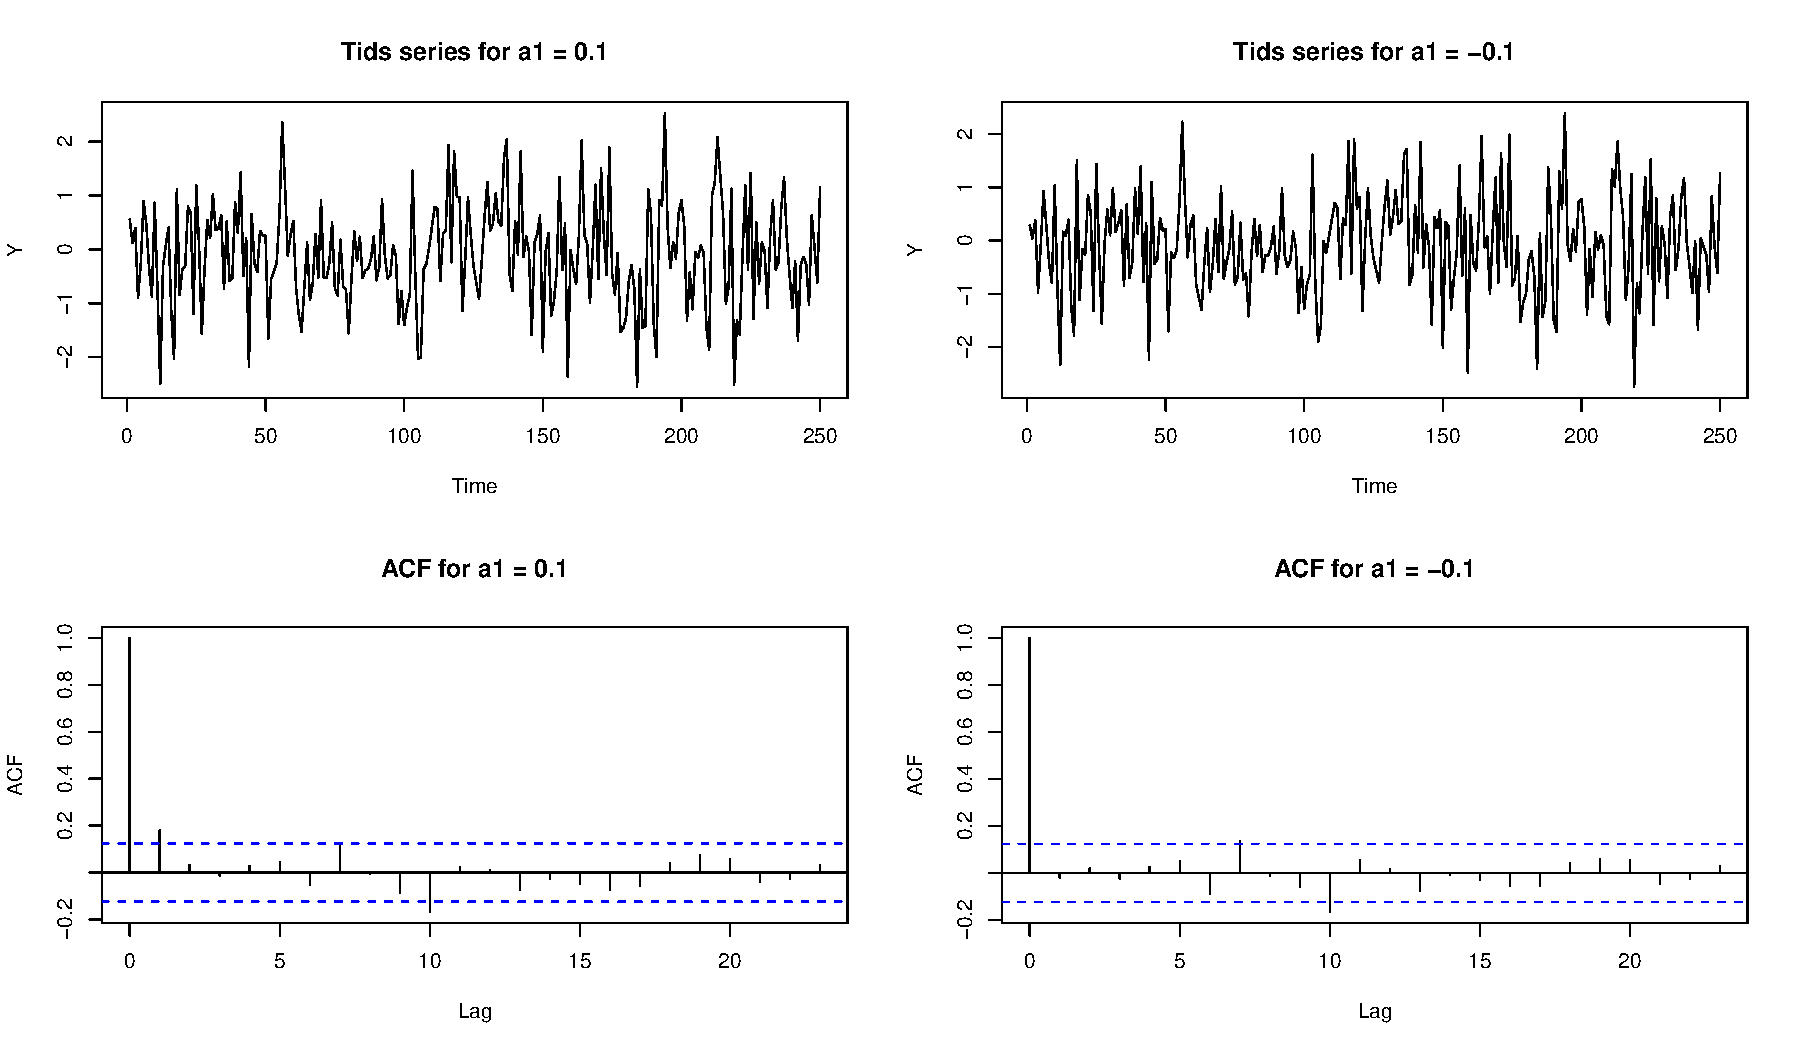
\includegraphics[width=140mm]{ar1-filter-1.pdf}
    \caption{Picture time}
    \label{fig:one}
\end{figure}

\begin{figure}
    \centering
    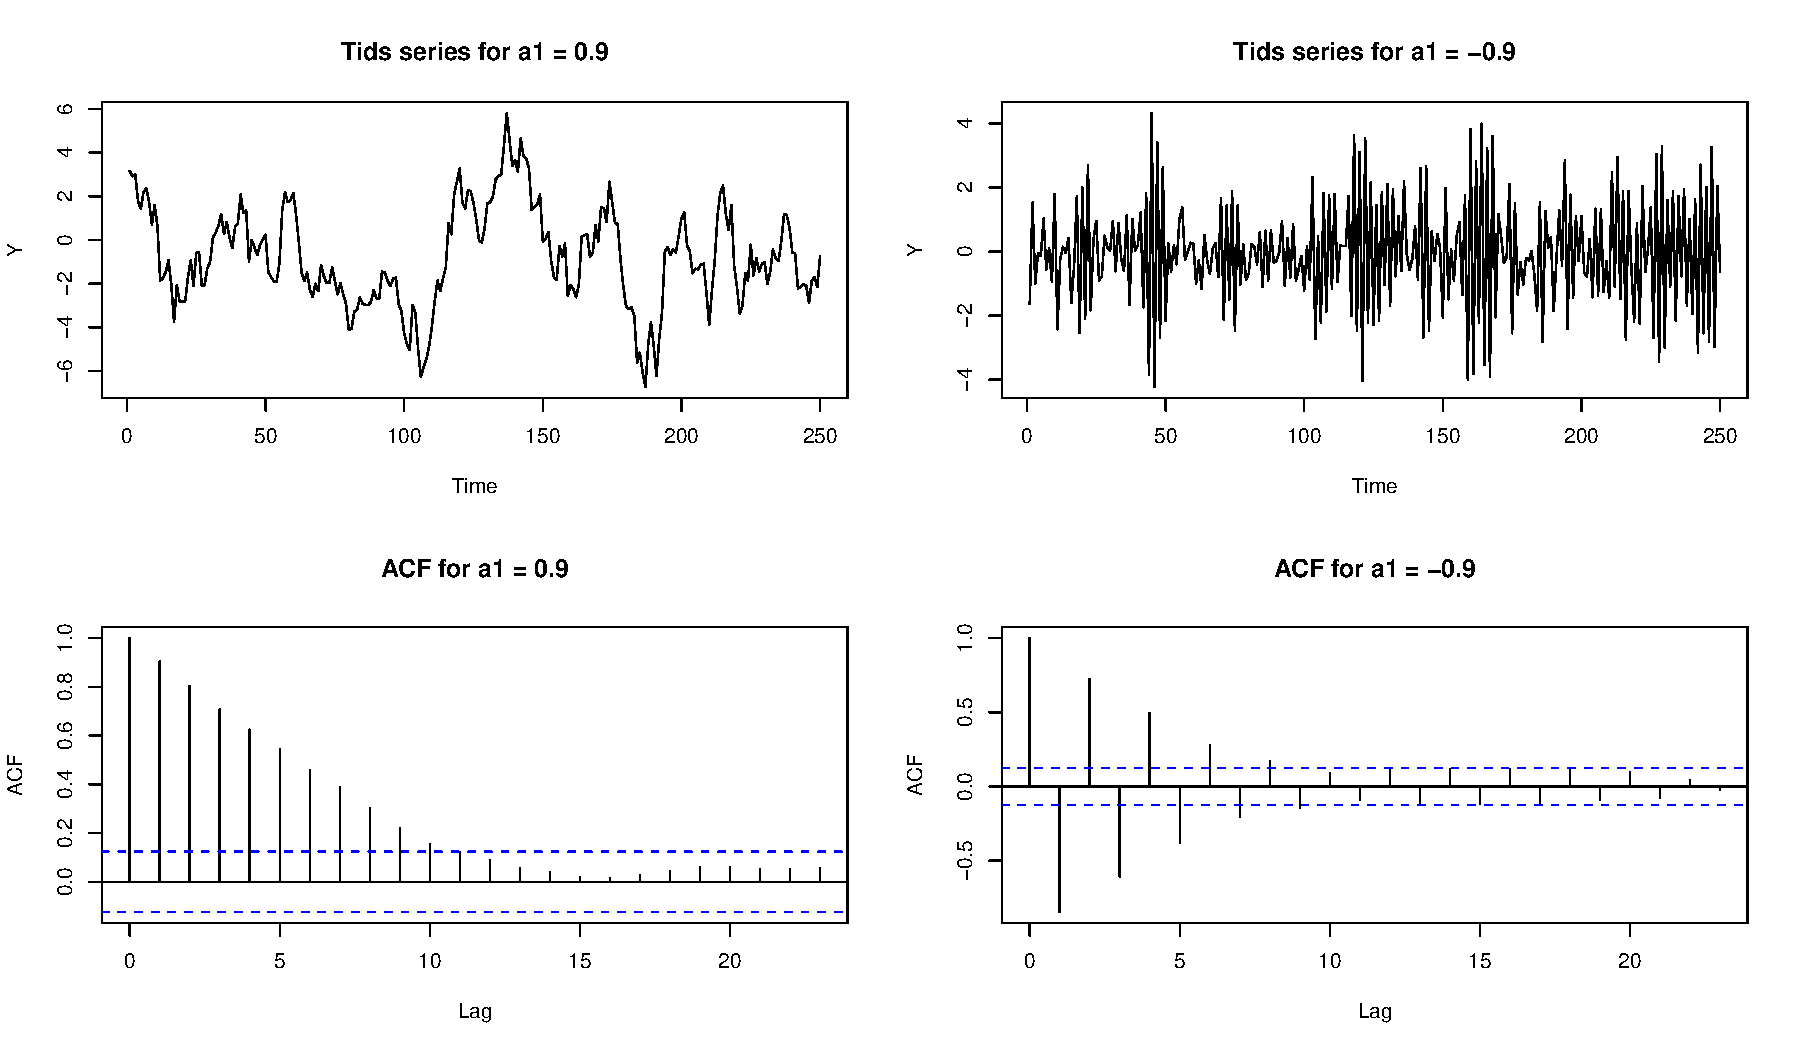
\includegraphics[width=140mm]{ar1-filter-2.pdf}
    \caption{Picture time}
    \label{fig:one}
\end{figure}

\begin{figure}
    \centering
    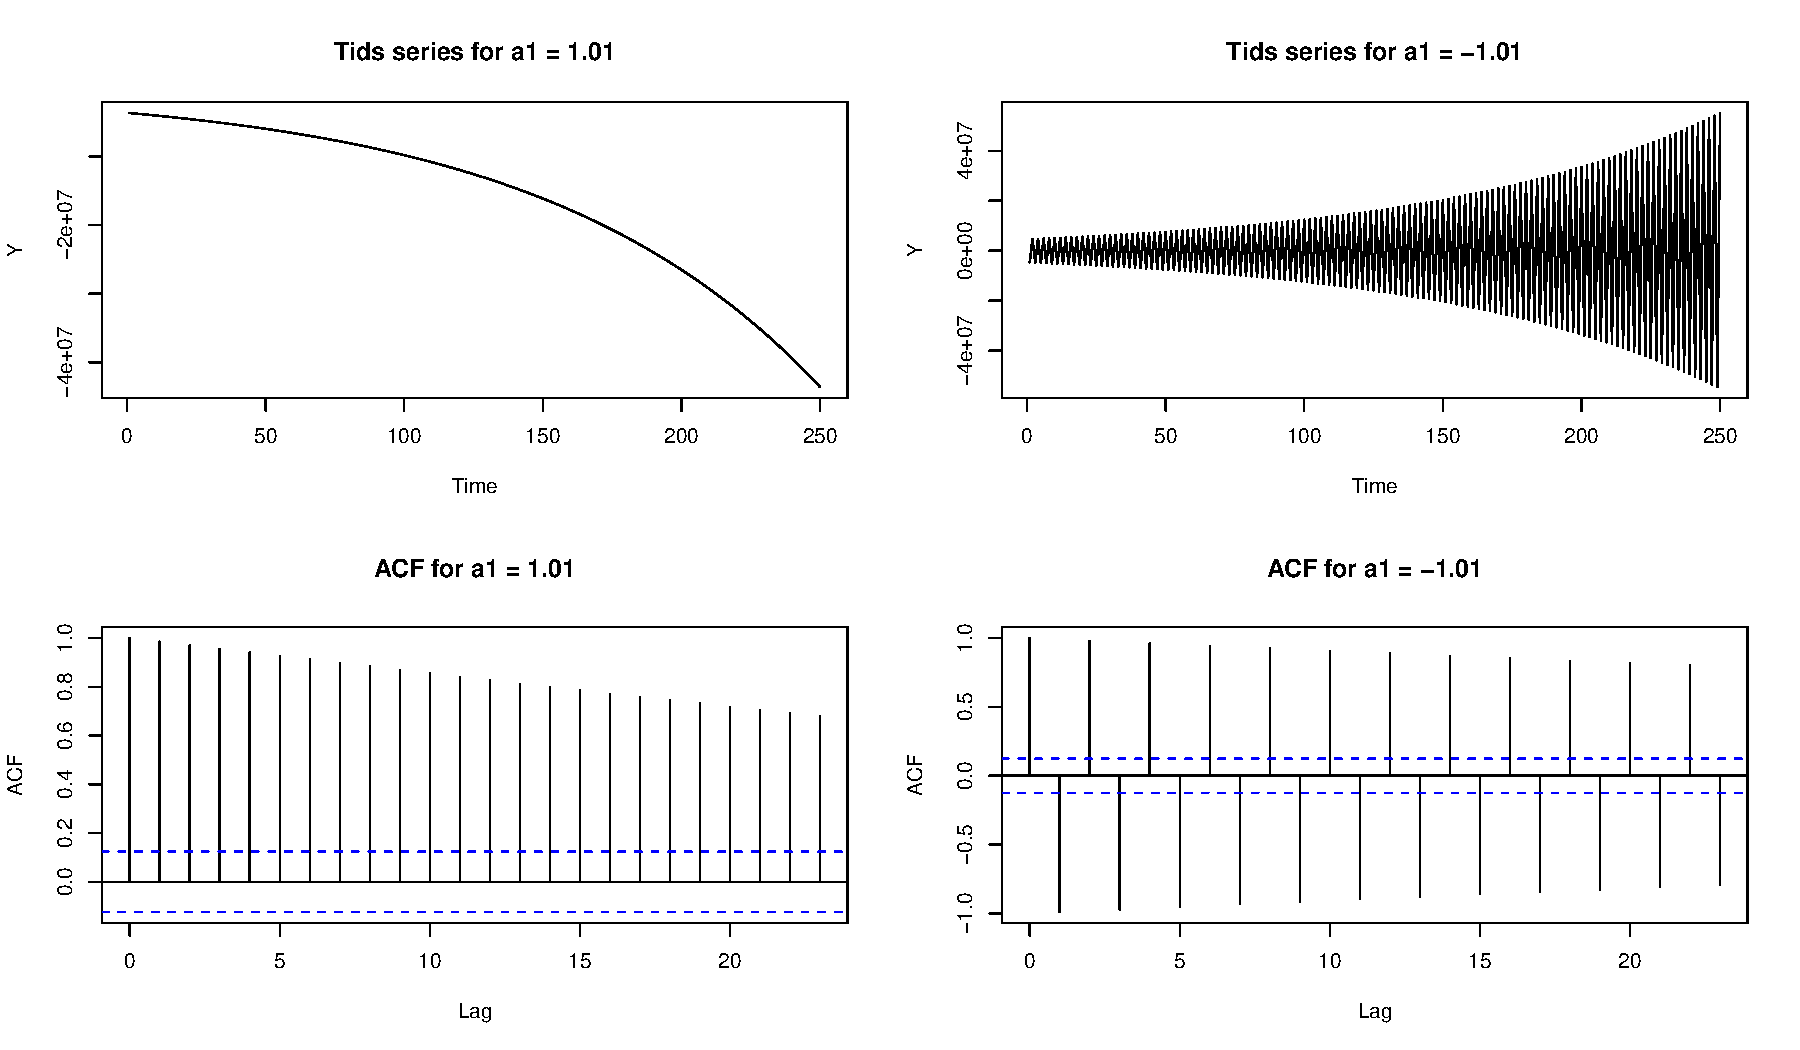
\includegraphics[width=140mm]{ar1-filter-3.pdf}
    \caption{Picture time}
    \label{fig:one}
\end{figure}


\begin{figure}
    \centering
    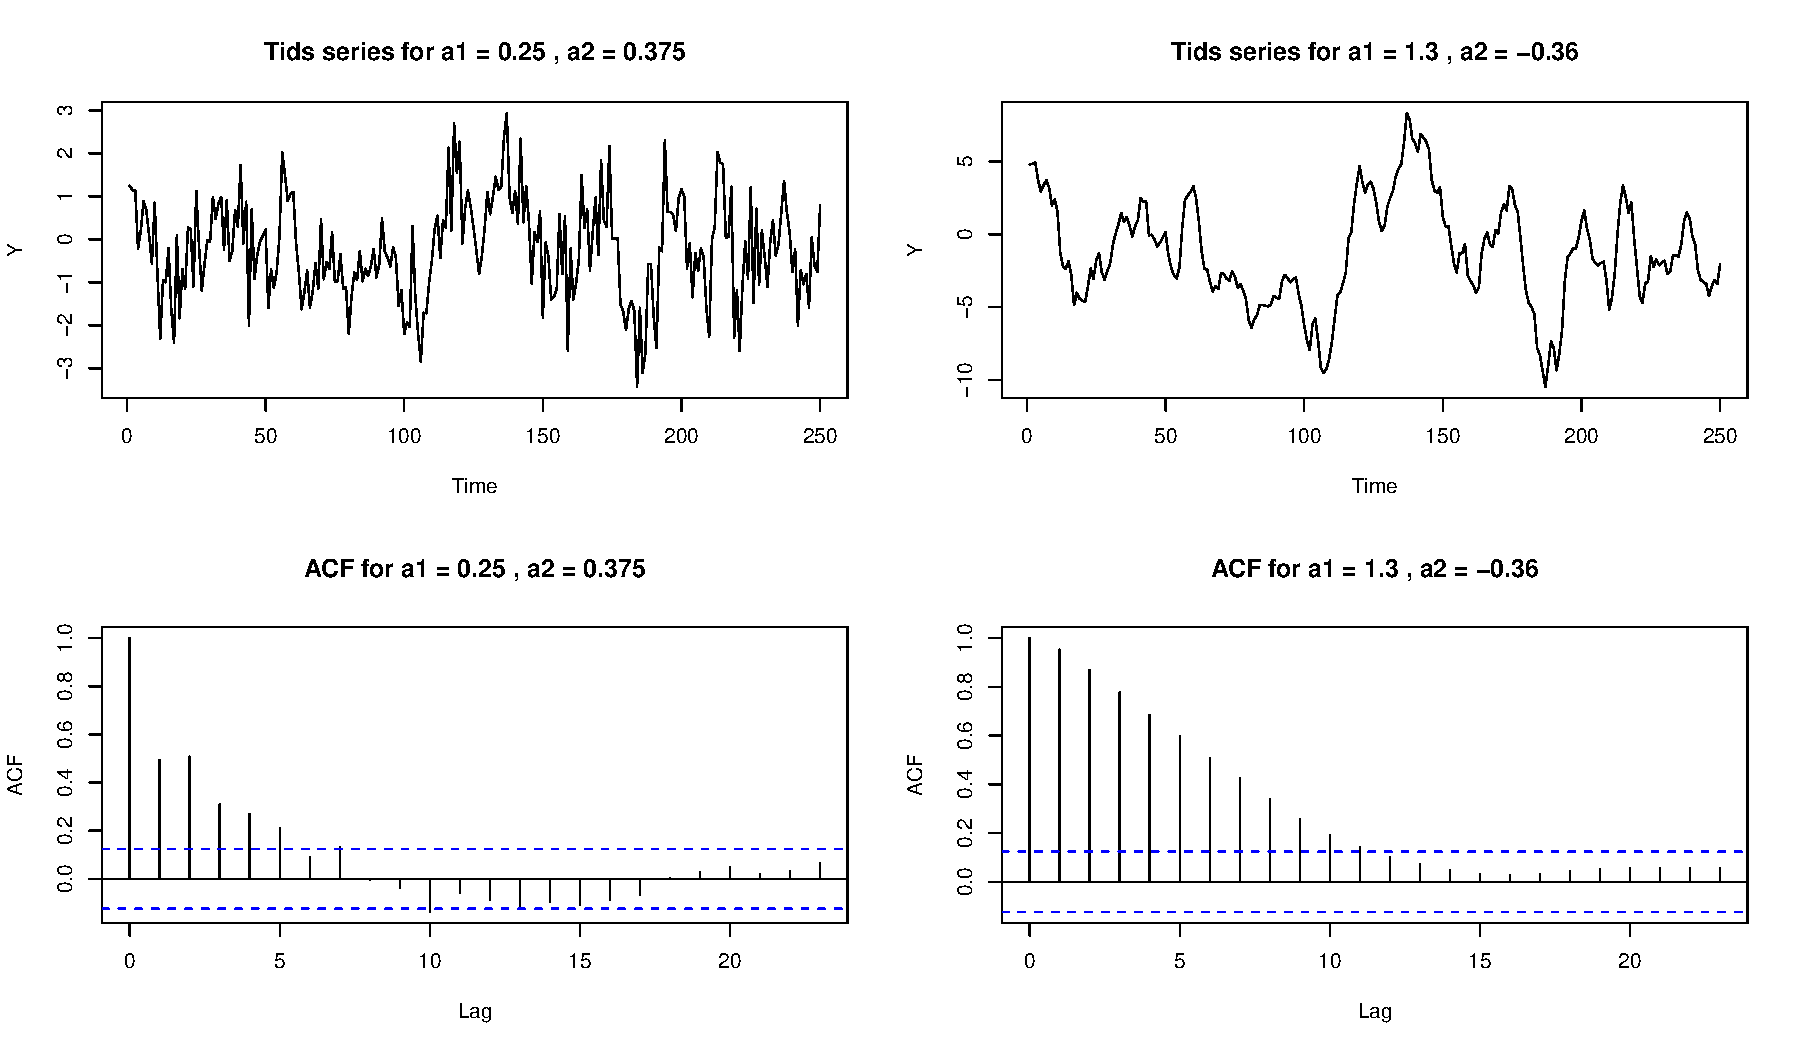
\includegraphics[width=140mm]{ar2-filter-1.pdf}
    \caption{Picture time}
    \label{fig:one}
\end{figure}

\begin{figure}
    \centering
    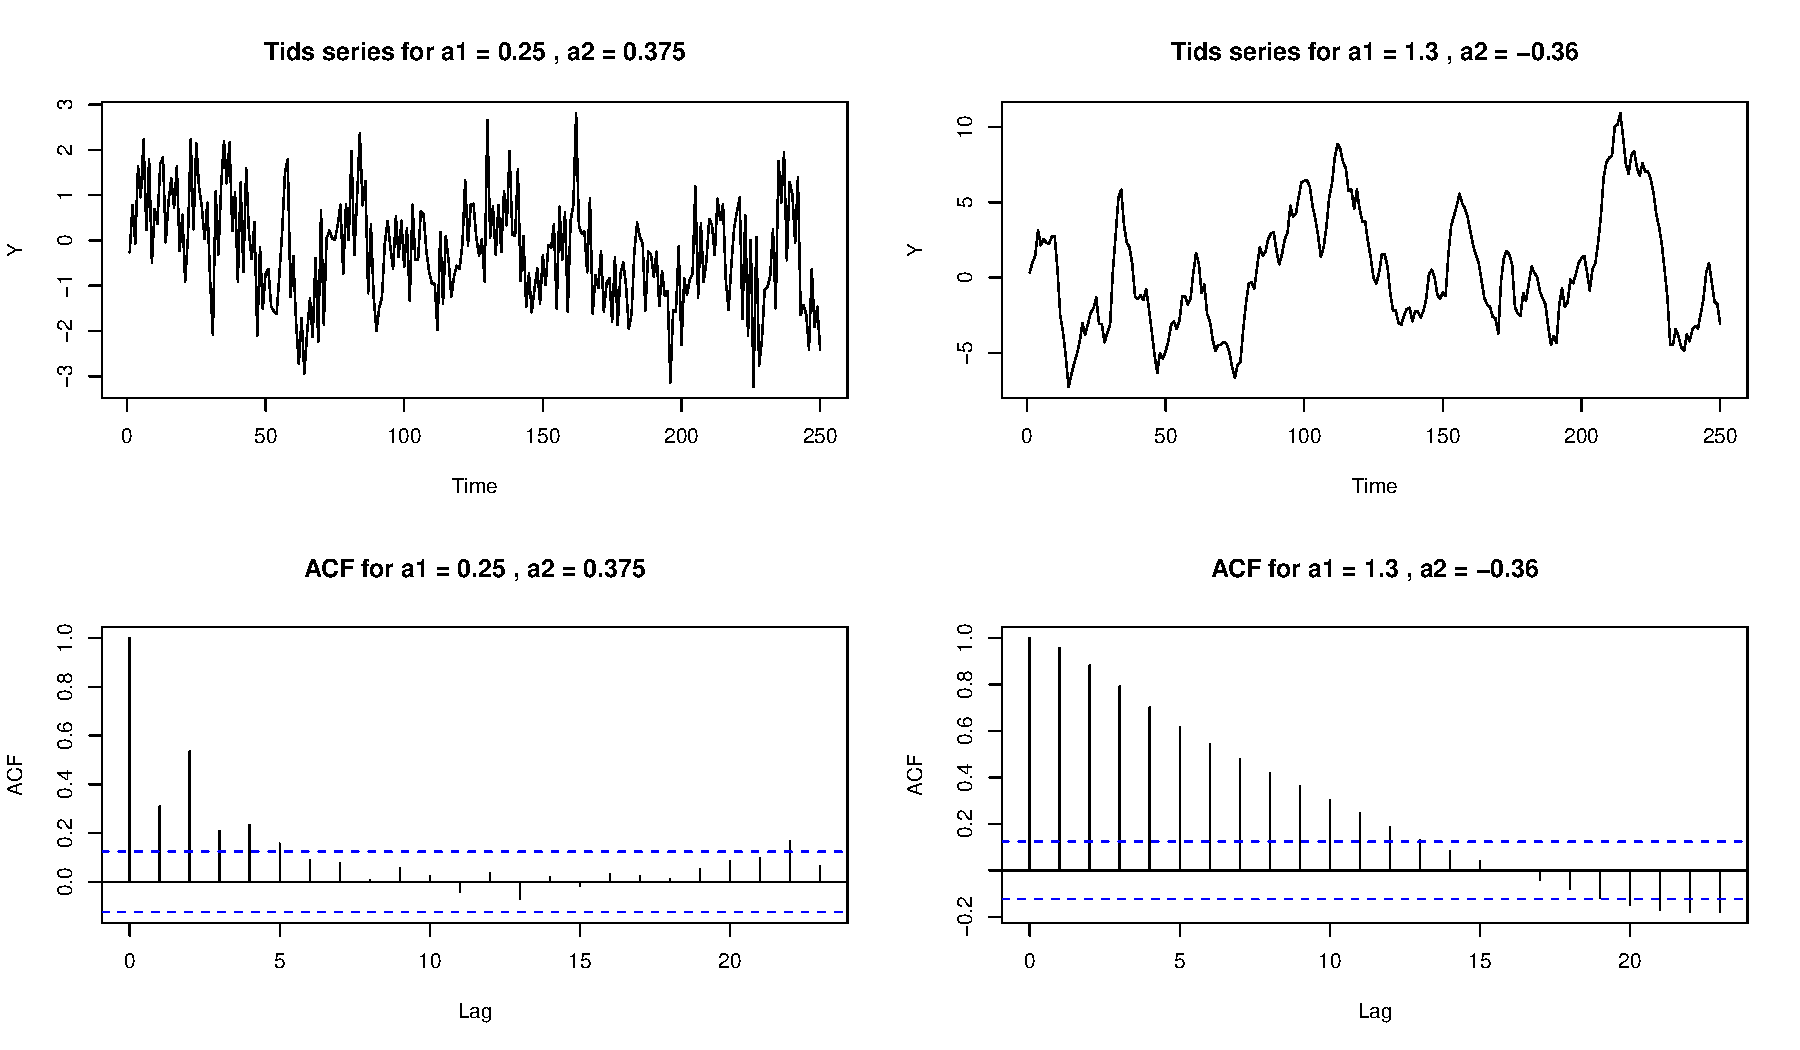
\includegraphics[width=140mm]{ar2-sim-1.pdf}
    \caption{Picture time}
    \label{fig:one}
\end{figure}

\pagebreak

\section*{Appendices}
All R code used for this assignment is included here. All source code incl. latex code for this report can be found at {\small\url{https://github.com/alphabits/dtu-fall-2011/tree/master/02417/assignment-2}}
\subsection*{(part2.R)}
\lstinputlisting{part2.R}

\begin{thebibliography}{9}

\bibitem{nocedal06}
  Jorge Nocedal \& Stephen J. Wright,
  \emph{Numerical Optimization}.
  Springer Science+Business Media,
  2nd Edition,
  2006.
\bibitem{nielsen10}
  Kaj Madsen \& Hans Bruun Nielsen,
  \emph{Introduction to Optimization and Data Fitting}.
  DTU IMM,
  1st Edition,
  2010.

\end{thebibliography}


\end{document}
